% Use only LaTeX2e, calling the article.cls class and 12-point type.

\documentclass[12pt]{article}

%Cosas copiadas del paper de Iñigo
\usepackage[table]{xcolor}
\RequirePackage{siunitx}
\RequirePackage[T1]{fontenc}                        % T1 font encoding for PDFs
\RequirePackage{lmodern}                                % extended font definition
\RequirePackage{amsmath,amssymb,amsthm} % most important math stuff
\RequirePackage{a4wide}                                 % make better use of A4 paper
\RequirePackage{fancyhdr}                               % custom headers and footers
\RequirePackage{fncychap}                               % custom chapter titles
\RequirePackage{graphicx}                               % graphics
\RequirePackage{color}                                  % color
\RequirePackage{booktabs}                               % extra tabular commands
\RequirePackage[format=plain]{caption}  % improved caption format
\RequirePackage{nomencl}                                % cool nomenclature listing
\RequirePackage{makeidx}                                % create your index
\RequirePackage[printonlyused]{acronym}
\RequirePackage{ifthen}                                 % if-then commands (used in maketitle)
\RequirePackage{eso-pic}                                % picture in back/forground (used in cover)
\RequirePackage{relsize}                                % \textlarger, \textsmaller etc
%%
%%
%%%%%%%%%%%%%%%%%%%%%%%%%%%%%%%%%%%%%%%%%%%%%%%%%%%%%%%%%%%%
%%
%%  Set up Matlab and C++ Listings
%%  REQUIRES PACKAGE listings AND colortbl
%%
%%%%%%%%%%%%%%%%%%%%%%%%%%%%%%%%%%%%%%%%%%%%%%%%%%%%%%%%%%%%
%%
%%

\RequirePackage{listings}%

\usepackage[utf8]{inputenc}

\usepackage{pgf,tikz}

\usepackage{pgfgantt}

\usepackage{mathrsfs}

\usepackage{mathtools}

\usepackage{gensymb}

\usepackage{float}

\usepackage{needspace}

\usepackage{pgfplots}

\usepackage[nodayofweek,level]{datetime}

\usepackage{todonotes}

\usepackage{bm}

\usepackage{enumitem}

\usepackage{graphicx}

\usepackage{subcaption}

\usepackage{indentfirst}

\usepackage{multirow}

\usepackage{eurosym}

\usepackage{hhline}

\usepackage{esvect}


\usepackage{upgreek}
\usepackage{arydshln}
\usepackage{algorithm}
\usepackage[noend]{algpseudocode}

\usepackage[nameinlink,capitalise]{cleveref}

\usepackage{mathtools}
%%%%%%%%%%% COPYPASTEADO DE GITHUB
\usepackage{amsmath}
\usepackage{amssymb}

\usepackage{wrapfig}

%redefine vector and Real symbols for faster typing
\renewcommand{\vec}[1]{\bm{#1}}
\newcommand{\R}{\mathbb R}
\newcommand{\Z}{\mathbb Z}
\newcommand{\foralli}[1][]{\forall i \in \{1\dots n_{#1}\}}
\newcommand{\forallj}[1][]{\forall j \in \{1\dots n_{#1}\}}
\newcommand{\forallk}[1][]{\forall k \in \{1\dots n_{#1}\}}
\newcommand{\dd}[2]{\frac{\partial #1}{\partial #2}}
\newcommand{\dt}[1]{\frac{d #1}{d t}}
\newcommand{\torque}{\tau}
\newcommand{\w}{\dot\varphi}
\newcommand{\h}{\frac{1}{2}}
\newcommand{\pare}[1]{\left(#1\right)}
\newcommand{\brac}[1]{\left\{#1\right\}}

\newcommand{\mat}[2][b]{\begin{#1matrix}#2\end{#1matrix}}

%set spacing between rows in tables
\renewcommand{\arraystretch}{1.2}

\def\F{\vec F}
\def\Torque{\vec \Gamma}
\def\R{\vec R}

\def\q{\vec q}
\def\M{\vec M}
\def\I{\vec I}
\def\C{\vec C}
\def\mults{\vec \lambda}

%   Fin de la parte copypasteada
\graphicspath{ {images/} }

% Users of the {thebibliography} environment or BibTeX should use the
% scicite.sty package, downloadable from *Science* at
% www.sciencemag.org/about/authors/prep/TeX_help/ .
% This package should properly format in-text
% reference calls and reference-list numbers.

\usepackage{scicite}

% Use times if you have the font installed; otherwise, comment out the
% following line.

\usepackage{times}

% The preamble here sets up a lot of new/revised commands and
% environments.  It's annoying, but please do *not* try to strip these
% out into a separate .sty file (which could lead to the loss of some
% information when we convert the file to other formats).  Instead, keep
% them in the preamble of your main LaTeX source file.


% The following parameters seem to provide a reasonable page setup.

\topmargin 0.0cm
\oddsidemargin 0.2cm
\textwidth 16cm 
\textheight 21cm
\footskip 1.0cm


%The next command sets up an environment for the abstract to your paper.

\newenvironment{sciabstract}{%
\begin{quote} \bf}
{\end{quote}}


% If your reference list includes text notes as well as references,
% include the following line; otherwise, comment it out.

\renewcommand\refname{References and Notes}

% The following lines set up an environment for the last note in the
% reference list, which commonly includes acknowledgments of funding,
% help, etc.  It's intended for users of BibTeX or the {thebibliography}
% environment.  Users who are hand-coding their references at the end
% using a list environment such as {enumerate} can simply add another
% item at the end, and it will be numbered automatically.

\newcounter{lastnote}
\newenvironment{scilastnote}{%
\setcounter{lastnote}{\value{enumiv}}%
\addtocounter{lastnote}{+1}%
\begin{list}%
{\arabic{lastnote}.}
{\setlength{\leftmargin}{.22in}}
{\setlength{\labelsep}{.5em}}}
{\end{list}}


% Include your paper's title here

\title{Geometric considerations of an alternative axes for Omnibot} 


% Place the author information here.  Please hand-code the contact
% information and notecalls; do *not* use \footnote commands.  Let the
% author contact information appear immediately below the author names
% as shown.  We would also prefer that you don't change the type-size
% settings shown here.

\author
{Siro Moreno$^{1\ast}$ \\
\\
\normalsize{$^{1}$Institut de Robótica i Informática Industrial}\\
\normalsize{dirección del IRI, Barcelona}\\
\normalsize{$^\ast$To whom correspondence should be addressed; E-mail:  ejemplo@ejemplo.eje}
}

% Include the date command, but leave its argument blank.

\date{}



%%%%%%%%%%%%%%%%% END OF PREAMBLE %%%%%%%%%%%%%%%%



\begin{document} 

% Double-space the manuscript.

\baselineskip24pt

% Make the title.

\maketitle 



% Place your abstract within the special {sciabstract} environment.

\begin{sciabstract}
  We will discuss some considerations and insights of using an alternative axes with the Omnibot robot, rotated 45 degrees respect to the symmetry axes.
\end{sciabstract}



% In setting up this template for *Science* papers, we've used both
% the \section* command and the \paragraph* command for topical
% divisions.  Which you use will of course depend on the type of paper
% you're writing.  Review Articles tend to have displayed headings, for
% which \section* is more appropriate; Research Articles, when they have
% formal topical divisions at all, tend to signal them with bold text
% that runs into the paragraph, for which \paragraph* is the right
% choice.  Either way, use the asterisk (*) modifier, as shown, to
% suppress numbering.

\section*{Definition of new axes}

\begin{wrapfigure}{l}{0.3\textwidth}
	\centering
	\includegraphics[width=\linewidth]{Omnibot_45_deg.png}
	\captionof{figure}{Omnibot new axes}
	\label{fig:omnibot}
\end{wrapfigure}
Let's define a new vector base system, anchored to the center of mass of the Omnibot and rotated 45 degrees clockwise respect to the B basis.
In order to describe the position of the wheels in this new base, we can define the magnitudes:
$$ l_2 = \frac{L-l}{\sqrt{2}}\ , \ L_2 = \frac{L+l}{\sqrt{2}}$$
We can follow the same process to calculate the equations of the system, but using the base 2 instead of the base B as an intermediate base between the $q_r$ and $q_w$ coordinates. We will also define $psi$ as the angle between the global X axis and the $x_2$ axis, instead of using the $x_B$ axis.

The first difference that we can observe is that using this base, some zeroes appear on the R matrix:

$$ R = \frac{\sqrt{2}}{r}\left[\begin{matrix}1 & 0 & - L_{2}\\0 & 1 & L_{2}\\0 & 1 & - L_{2}\\1 & 0 & L_{2}\end{matrix}\right]$$

We observe that movement on $x_2$ and $y_2$ uncouples.

\subsection*{Definition of $\vec{w}$ and $\vec{a}$ }

Let's define two new concepts: $\vec{w}$ and $\vec{a}$:

$$ \vec{w} \equiv \left[\begin{matrix} w_1\\w_2\\\dot{\psi}\end{matrix}\right] \equiv \R_{\psi}^T \dot{\q_r}\ ,\ \vec{a} \equiv \left[\begin{matrix} a_1\\a_2\\\ddot{\psi}\end{matrix}\right] \equiv \R_{\psi}^T \ddot{\q_r}$$

We observe that  $\vec{w}$ and $\vec{a}$ are the proyection on base 2 of the global speeds and accelerations of the robot's center of mass. We must be cautious when using them, because since $\R_{\psi}$ can vary with time, in general $\frac{d\vec{w}}{dt}\neq\vec{a}$.
$$\frac{d\vec{w}}{dt} = \frac{d(\R_{\psi}^T \dot{\q_r})}{dt} =  \frac{d(\R_{\psi}^T)}{dt}\dot{\q_r} + \R_{\psi}^T \ddot{\q_r}=  \frac{d(\R_{\psi}^T)}{dt}\dot{\q_r} + \vec{a}$$

Why are then these variables useful? The answer begins with the relationship that connects  $\vec{w}$ and $\dot{\q_w}$:
$$\dot{\q_w} = \R \R_{\psi}^T \dot{\q_r} = \R \vec{w} = \frac{\sqrt{2}}{2}\left[\begin{matrix}- L_{2} \dot{\psi} + w_1\\L_{2} \dot{\psi} + w_2\\- L_{2} \dot{\psi} + w_2\\L_{2} \dot{\psi} + w_1\end{matrix}\right]$$
We can observe from this that rotation of wheels 1 and 4 only depend on $\dot{\psi}$ and $w_1$, while rotation of wheels 2 and 3 only depend on $\dot{\psi}$ and $w_2$.

This means that, as the speed of the robot is limited by the maximum speed in any of its wheels' shafts, the envelope of achievable speeds in $x_2$ and $y_2$ will always be a square whose size depends on $\dot{\psi}$:
\begin{figure}[h]
	\centering
	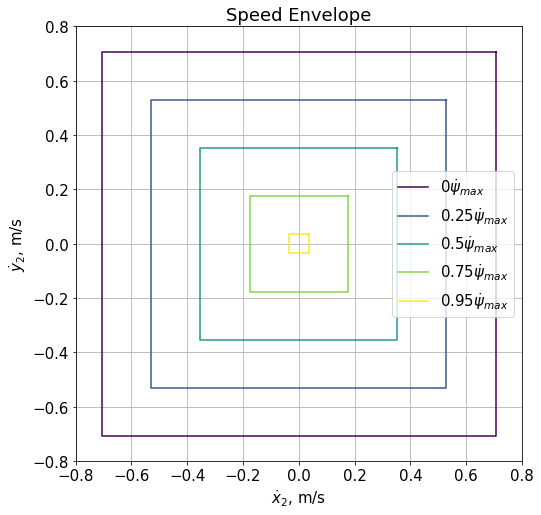
\includegraphics[width=.5\linewidth]{speed_envelope}
	\captionof{figure}{Speed Envelope}
	\label{fig:speed_envelope}
\end{figure}

\section*{Proyection of the equation}

As we know from the work of Iñigo, we can describe the Omnibot system dynamics as
\begin{gather}
	\vec H \ddot \q_r+ \vec K \dot \q_r=\R_{\psi}\R ^T\Torque \label{eq:solution}
\end{gather}
Where:
\begin{gather}
	\vec H = \mat{ m+\frac{4\,I_w}{r^2} & 0 & 0 \\ 0 & m+\frac{4\,I_w}{r^2} & 0 \\ 0 & 0 & I_z+\frac{4\,I_w\,{\left(L+l\right)}^2}{r^2} } \label{eq:H}
	\\
	\vec K = \mat{ 0 & \frac{4\,I_w\,\dot \psi }{r^2} & 0 \\ -\frac{4\,I_w\,\dot \psi }{r^2} & 0 & 0 \\ 0 & 0 & 0 }
\end{gather}

By definition: $ \dot{\q}_2  = \R_{\psi}^T \dot{\q_r}\ ,\ \ddot{\q}_2 = \R_{\psi}^T \ddot{\q_r}$

Which means that also $ \dot{\q}_r  = \R_{\psi} \vec{w}\ ,\ \ddot{\q}_r = \R_{\psi} \vec{a}$

So we can rewrite the system's equation as
$$	\vec H \R_{\psi} \vec{a}+ \vec K \R_{\psi} \vec{w}=\R_{\psi}\R ^T\Torque$$

Multiplying the whole equation leftside by $\R_{\psi}^T$, we get:
$$ \R_{\psi}^T	\vec H \R_{\psi} \vec{a}+ \R_{\psi}^T \vec K \R_{\psi} \vec{w}=\R ^T\Torque$$
Operating, we find that $\R_{\psi}^T	\vec H \R_{\psi} = \vec{H}$ and $\R_{\psi}^T \vec{K} \R_{\psi} = \vec{K}$, so our equation proyected on axes 2 becomes:
\begin{gather}
\vec H \ddot \q_2+ \vec K \dot \q_2=\R ^T\Torque \label{eq:axes_2_eq}
\end{gather}
We can use this equation to gain more insight on the nature of the system.

\section*{Electric power}
\subsection*{Constant movement without rotation}
Let's start by assuming a straight uniform movement without rotation:
$$ \vec{w} = \left[\begin{matrix}w_1\\w_2\\0\end{matrix}\right]\ ,\ \dot{\q_w} = \R \vec{w} = \frac{\sqrt{2}}{r} \left[\begin{matrix}w_1\\w_2\\w_2\\w_1\end{matrix}\right]$$

We remember that the electric motor model looks like this:
$$ V = K_m N\dot{\phi} + Ri$$
$$ \tau_m = N K_ei\mu_{trans} - \tau_r$$
$$ \tau_r = a \dot{\phi} + b\operatorname{sign}(\dot{\phi}) $$
And that in straight constant movement the torque output is zero, so that the electric power consumed in a motor is 
$$ P_m = 0.301 \operatorname{sign}^{2}\left(\dot{\phi}\right) + 0.638 \operatorname{sign}\left(\dot{\phi}\right) \dot{\phi} + 0.016 \dot{\phi}^{2}$$
We can add the power consumed by all four motors to get 
$$P_{tot} = 0.6 \operatorname{sign}^{2}\left(w_1\right) + 27.05 \operatorname{sign}\left(w_1\right) w_1 + 0.6 \operatorname{sign}^{2}\left(w_2\right) + 27.05 \operatorname{sign}\left(w_2\right) w_2 + 14.17 w_1^{2} + 14.17 w_2^{2}$$

Which we can plot over $w_1$ and $w_2$: 
\begin{figure}[h]
	\centering
	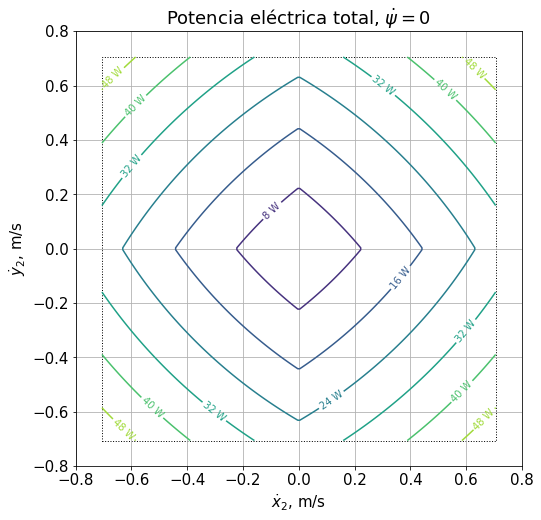
\includegraphics[width=.5\linewidth]{power_map_base_2}
	\captionof{figure}{Total electric power required to keep constant speed}
	\label{fig:power_ct_speed}
\end{figure}

We can observe that movement is most efficient in the $x_2$ and $y_2$ directions, when only two motors are running, while the least efficient directions are rotated 45 degrees respect to them: the symmetry axes of the robot.
\subsection*{Constant movement with rotation}
If our robot keeps a straight movement with constant rotation rate:
$$ \vec{a} = \vec{0}\ ,\ \vec{w} = \left[\begin{matrix}w_1\\w_2\\\dot{\psi}\end{matrix}\right]\ ,\ \dot{\q_w} = \R \vec{w} = \frac{\sqrt{2}}{r} \left[\begin{matrix}- L_{2} \dot{\psi} + w_1\\L_{2} \dot{\psi} + w_2\\- L_{2} \dot{\psi} + w_2\\L_{2} \dot{\psi} + w_1\end{matrix}\right]$$

Subtituting in the General equation:

$$\vec H \ddot \q_2+ \vec K \dot \q_2=\vec K \dot \q_2=\R ^T\Torque$$

Multiplying the equation leftside by $\R^{-1T}$:
$$\Torque=\R^{-1T}\vec K \dot \q_2 = \frac{\sqrt{2}I_w}{r}\left[\begin{matrix}\dot{\psi} w_2\\- \dot{\psi} w_1\\- \dot{\psi} w_1\\\dot{\psi} w_2\end{matrix}\right]$$

Now the torque is not zero, but we can use the model to get an expression that models the electric power of a motor as a function of the torque $\tau_m$ and the angular speed $\dot{\phi}$:
$$P_m = \left(\frac{K_{m} a}{K_{e} \mu} + \frac{R_{e} a^{2}}{K_{e}^{2} \mu^{2} n^{2}}\right) \dot{\phi}^{2} + \left(\frac{K_{m} b \operatorname{sign}\left(\dot{\phi}\right)}{K_{e} \mu} + \frac{K_{m} \tau_{m}}{K_{e} \mu} + \frac{2 R_{e} a b \operatorname{sign}\left(\dot{\phi}\right)}{K_{e}^{2} \mu^{2} n^{2}} + \frac{2 R_{e} a \tau_{m}}{K_{e}^{2} \mu^{2} n^{2}}\right) \dot{\phi} +$$
$$+ \frac{R_{e} b^{2} \operatorname{sign}^{2}\left(\dot{\phi}\right)}{K_{e}^{2} \mu^{2} n^{2}} + \frac{2 R_{e} b \tau_{m} \operatorname{sign}\left(\dot{\phi}\right)}{K_{e}^{2} \mu^{2} n^{2}} + \frac{R_{e} \tau_{m}^{2}}{K_{e}^{2} \mu^{2} n^{2}}$$
Or, subtituting the constants with their values:
$$ P_m = 1.881 \tau_{m}^{2} + 1.505 \tau_{m} \operatorname{sign}\left(\dot{\phi}\right) + \left(1.594 \tau_{m} + 0.638 \operatorname{sign}\left(\dot{\phi}\right)\right) \dot{\phi} + 0.301 \operatorname{sign}^{2}\left(\dot{\phi}\right) + 0.016 \dot{\phi}^{2}$$

If we add the power spent by the four motors substituting in this expression $\tau_m$ and $\dot{\phi}$ by its values functions of $q_2$, we get a function that expresses the total electric power as a function of $w_1$, $w_2$ and $\dot{\psi}$:
\begin{multline}
P_{tot} = \displaystyle 0.3 \operatorname{sign}^{2}\left(4.44 \dot{\psi} - 14.99 w_1\right) - 0.08 \operatorname{sign}\left(4.44 \dot{\psi} - 14.99 w_1\right) \dot{\psi} w_2 + \\+4.01 \operatorname{sign}\left(4.44 \dot{\psi} - 14.99 w_1\right) \dot{\psi} - 13.52 \operatorname{sign}\left(4.44 \dot{\psi} - 14.99 w_1\right) w_1 + 0.3 \operatorname{sign}^{2}\left(4.44 \dot{\psi} + 14.99 w_1\right) +\\+ 0.08 \operatorname{sign}\left(4.44 \dot{\psi} + 14.99 w_1\right) \dot{\psi} w_2 + 4.01 \operatorname{sign}\left(4.44 \dot{\psi} + 14.99 w_1\right) \dot{\psi} + 13.52 \operatorname{sign}\left(4.44 \dot{\psi} + 14.99 w_1\right) w_1 +\\+ 0.3 \operatorname{sign}^{2}\left(4.44 \dot{\psi} - 14.99 w_2\right) + 0.08 \operatorname{sign}\left(4.44 \dot{\psi} - 14.99 w_2\right) \dot{\psi} w_1 + 4.01 \operatorname{sign}\left(4.44 \dot{\psi} - 14.99 w_2\right) \dot{\psi} -\\- 13.52 \operatorname{sign}\left(4.44 \dot{\psi} - 14.99 w_2\right) w_2 + 0.3 \operatorname{sign}^{2}\left(4.44 \dot{\psi} + 14.99 w_2\right) - 0.08 \operatorname{sign}\left(4.44 \dot{\psi} + 14.99 w_2\right) \dot{\psi} w_1 +\\+ 4.01 \operatorname{sign}\left(4.44 \dot{\psi} + 14.99 w_2\right) \dot{\psi} + 13.52 \operatorname{sign}\left(4.44 \dot{\psi} + 14.99 w_2\right) w_2 + 0.01 \dot{\psi}^{2} w_1^{2} + 0.01 \dot{\psi}^{2} w_2^{2} +\\+ 2.49 \dot{\psi}^{2} + 14.17 w_1^{2} + 14.17 w_2^{2}
\end{multline}
While certainly not very beautiful, this expression contains a lot of information about the influence of the parameters in power consumption. For example, plotting the power over $w_1$ and $w_2$ for different $\dot{\psi}$:
\begin{figure}[h]
	\centering
	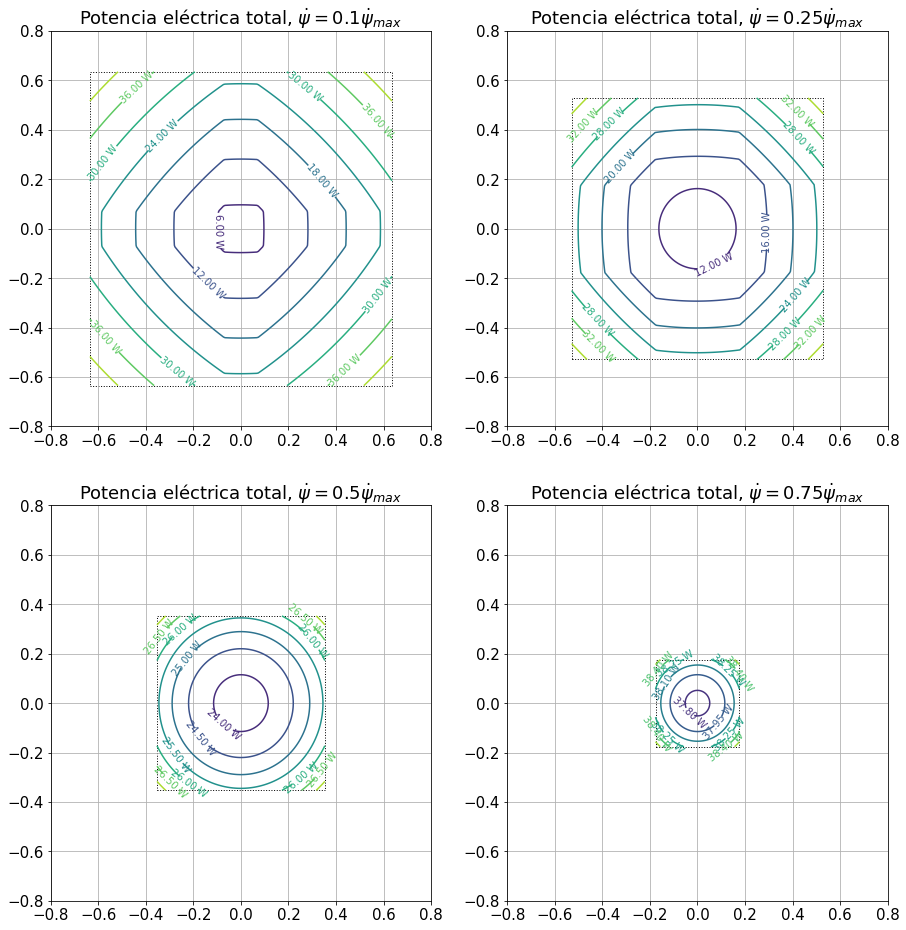
\includegraphics[width=.9\linewidth]{power_map_base_2_psi_dot}
	\captionof{figure}{Total electric power required to keep constant speed}
	\label{fig:power_ct_speed_psi_dot}
\end{figure}

We can also try to understand beter this 3-D relationship by slicing through a plane where $w_2=0$ or where $w_1 = w_2$:
\begin{figure}[h]
	\centering
	\begin{minipage}{.5\textwidth}
		\centering
		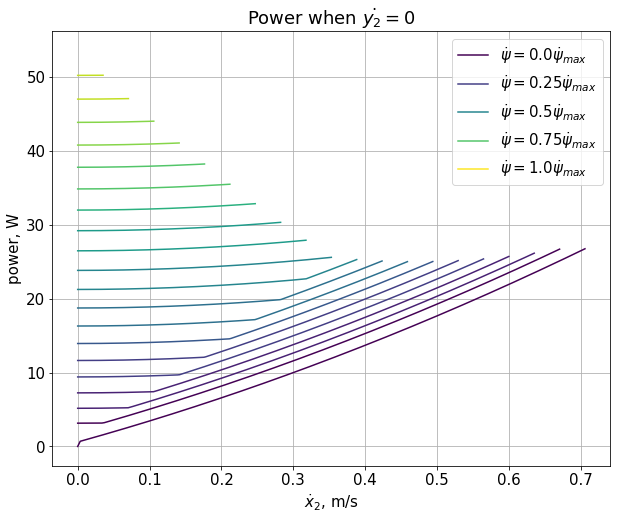
\includegraphics[width=.9\linewidth]{power_map_y_0}
		\label{fig:power_y_0}
	\end{minipage}%
	\begin{minipage}{.5\textwidth}
		\centering
		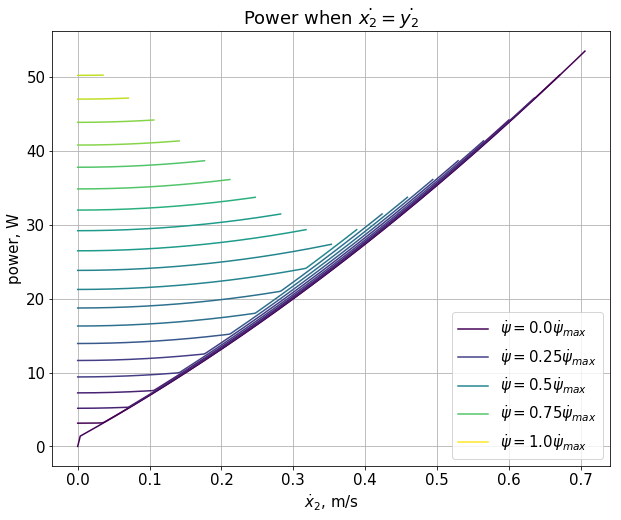
\includegraphics[width=.9\linewidth]{power_map_y_x}
		\label{fig:power_y_x}
	\end{minipage}
\end{figure}

We can use a combination of both kinds of graphs to see, for example, how power compsumption slowly becomes independent of direction as $\dot{\psi}$ increases, or how the two conditions that spend maximum power are when all the four wheels turn at their maximum speed, either moving the robot in a straight line or rotating in place. We can also check that when $\dot{\psi} = 0$, for any given $w_1$, the power compsumption when $w_1 = w_2$ is exactly twice as when $w_2=0$, even though the total speed achived is only $\sqrt{2}$ times larger.
\section*{Conclusions}

We have used the new axes base 2 to gain meaningful insights and understandings of how the Omnibot works and moves.
% Your references go at the end of the main text, and before the
% figures.  For this document we've used BibTeX, the .bib file
% scibib.bib, and the .bst file Science.bst.  The package scicite.sty
% was included to format the reference numbers according to *Science*
% style.


%\bibliography{scibib}

%\bibliographystyle{Science}



% Following is a new environment, {scilastnote}, that's defined in the
% preamble and that allows authors to add a reference at the end of the
% list that's not signaled in the text; such references are used in
% *Science* for acknowledgments of funding, help, etc.

%\begin{scilastnote}
%\item We've included in the template file \texttt{scifile.tex} a new
%environment, \texttt{\{scilastnote\}}, that generates a numbered final
%citation without a corresponding signal in the text.  This environment
%can be used to generate a final numbered reference containing
%acknowledgments, sources of funding, and the like, per {\it Science\/}
%style.
%\end{scilastnote}




% For your review copy (i.e., the file you initially send in for
% evaluation), you can use the {figure} environment and the
% \includegraphics command to stream your figures into the text, placing
% all figures at the end.  For the final, revised manuscript for
% acceptance and production, however, PostScript or other graphics
% should not be streamed into your compliled file.  Instead, set
% captions as simple paragraphs (with a \noindent tag), setting them
% off from the rest of the text with a \clearpage as shown  below, and
% submit figures as separate files according to the Art Department's
% instructions.


%\clearpage

%\noindent {\bf Fig. 1.} Please do not use figure environments to set
%up your figures in the final (post-peer-review) draft, do not include graphics in your
%source code, and do not cite figures in the text using \LaTeX\
%\verb+\ref+ commands.  Instead, simply refer to the figure numbers in
%the text per {\it Science\/} style, and include the list of captions at
%the end of the document, coded as ordinary paragraphs as shown in the
%\texttt{scifile.tex} template file.  Your actual figure files should
%be submitted separately.



\end{document}




















